\chapter{РАЗРАБОТКА ПРОГРАММНОЙ СРЕДЫ}



\section{Итоговая архитектура среды}

Прежде чем приступить к разработке среды, подробно опишем её компоненты, связи между этими компонентами и соответствующией функции.

Среда~--- это программная система, которая состоит из двух основных модулей. Чтобы различать их, перечислим их и присвоим каждому название:
\begin{itemize}
\item модуль управления ходом испытания \textit{Kyzylborda\footnotemark[1];}
\item модуль, предоставляющий участникам среду для прохождения испытаний \textit{SchoolOS}.
\end{itemize}

\footnotetext[1]{Название системы придумано другим членом оргкомитета и является каламбуром: с одной стороны, этот модуль реализует то, что называют словом <<борда>>, с другой~--- существует известный казахстанский город Кызылорда, и эти слова рифмуются. Упустить такой шанс было невозможно.}
\Abbrev{HTTP}{(англ. hypertext transfer protocol) протокол передачи гипертекста}
\Abbrev{UML}{(англ. unified modeling language) единый язык для моделирования}

Архитектуру среды можно описать на языке диаграмм UML \textit{(англ. unified modeling language, единый язык для моделирования).} UML~--- это открытый стандарт, позволяющий создавать графическое представление сложных систем на разных уровнях: от глобального межсистемного взаимодействия до локальных сценариев использования конкретных компонент \cite{UML}.

Для описания архитектуры была составлена т.н. диаграмма пакетов (рисунок \ref{fig:uml-model}), отражающая связи между произвольными группами сущностей, объединёнными семантически, т.е. \textit{пакетами.} В данном случае в роли пакетов выступают системы и подсистемы среды. Пунктирными стрелками устанавливается отношение <<пакет зависит от>>: так устанавливаются абстрактные функциональные связи.

\Define{Пакет (в UML)}{механизм общего назначения в языке UML для группировки элементов по семантическим связям в целях обеспечения наглядности структуры модели системы}

\begin{figure}[h]
  \centering
  \includegraphics[width=1\textwidth]{inc/dia/uml-model.eps}
  \caption{UML-диаграмма пакетов для среды}
  \label{fig:uml-model}
\end{figure}

Модуль Kyzylborda~--- это клиент-серверное приложение с веб-интерфейсом, то есть приложение, доступ к которому осущесвтляется пользователями по протоколу HTTP \textit{(англ. hyptertext transfer protocol, протокол передачи гипертекста).} Оно состоит из модуля задач и модуля, предоставляющего веб-интерфейс.

Модуль SchoolOS~--- это дистрибутив ОС Linux, содержащий в себе клиент-серверные компоненты, реализующие функциональность, связанную с провизией и прокторингом, а также предоставляющий доступ участника к ВМ с гостевой ОС.

Пакеты этих модулей были декомпозированы с учётом функций, описанных в Главе 2. В ходе дальнейшей разработки декомпозиция будет продолжена.

Оба модуля так или иначе должны взаимодействовать с уже существующей ИС <<Юрт>>, используемой оргкомитетом для регистрации участников и обработки их персональных данных. Интеграция с ИС в случае модуля Kyzylborda необходима для обеспечения аутентификации участников, в случае SchoolOS~--- для получения сведений о них и о проводимом испытании.

Описание разработки модулей будет производиться в обратном порядке, чем в предыдущей главе. Это связано с тем, что технологию NixOS, используемую в обоих модулях, лучше начать рассматривать с примеров, связанных с её непосредственным назначением~--- управлением конфигурацией ОС, которые возникнут при разработке SchoolOS.

\FloatBarrier

\section{Модуль среды SchoolOS}

Технологическая основа для данного модуля~--- базовая операционная система. В Главе 2 для этой роли был выбран дистрибутив ОС Linux, NixOS, построенный вокруг функционального декларативного пакетного менеджера Nix.

NixOS позволяет описать состояние ОС целиком как будто это состояние~--- ещё один пакет, подлежащий установке. Такой подход позволяет обеспечить, во-первых~--- воспроизводимость сборки конфигурации, во-вторых~--- её неизменчивость (иммутабельность). Любые изменения, вносимые в конфигурацию применяются подобно транзакциям, порождая каждый раз новую версию ОС, а не производятся <<наживую>>, как это реализовано в традиционных пакетных менеджерах.

С помощью конфигурации NixOS можно определить системные параметры, включая параметры загрузки и настройки разграничения доступа, набор установленного ПО, (а также само ПО как пакет, если речь идёт о самостоятельно разработанных программах), перечень системных сервисов и прочие нюансы.

В предыдущем разделе отмечалось, что модули, обеспечивающие прокторинг и провизию, требуют клиент-серверной архитектуры, причём взаимодействие сторон должно осуществляться по протоколу SSH. NixOS позволяет также разработать и конфигурацию ОС для сервера, упростив и автоматизировав процесс его развёртывания в дальнейшем.

Сами модули для прокторинга и провизии стоит разработать как набор скриптов для командной оболочки ОС Linux, поскольку их реализация не подразумевает сложных алгоритмов, но требует постоянного взаимодействия с разными частями базовой ОС~--- напрмер, захват экрана, создание SSH-туннелей и т.п.

Таким образом, для имплементации модуля SchoolOS необходимо:
\begin{enumerate}
\item
  разработать модули провизии и прокторинга;
\item
  разработать конфигурацию NixOS для базовой ОС (клиент);
\item
  разработать конфигурацию NixOS для серверной ОС.
\end{enumerate}

\subsection{Подмодуль провизии и прокторинга}

Определим протокол взаимодействия клиента и сервера и способ соединения. Для целей провизии, центральному серверу необходимо получать актуальную и полную картину того, какие клиенты к нему подключены~--- это также следует предусмотреть при разработке подмодуля.

Кроме того, необходимо, чтобы провизия осуществлялась в ручном режиме на случай сбоев.

\subsubsection{Протокол клиент-серверного взаимодействия}

С помощью SSH можно выполнять команды на удалённой машине. При этом, открывается сеанс в командной оболчке пользователя, от имени которого осуществляется доступ.

Де-факто стандартная имплементация SSH, программа OpenSSH, позволяет изменить это поведение. Можно настроить сервер так, чтобы при подключении выполнялась одна и та же команда независимо от того, с каким запросом подключился клиент. То есть, если, например, указать в параметрах сервера следующую директиву \texttt{command="/bin/date"}, то при подключении к нему по SSH клиент получит только текущую дату, после чего программа завершится.

Этот механизм позволяет безопасно реализовать обработчик подключений. Более того, при работе в таком режиме, в окружение сервера передаётся переменная окружения \texttt{SSH\_ORIGINAL\_COMMAND}, из которой можно получить данные <<запроса>> клиента.

Клиенты должны однозначно идентифицироваться и содержать данные о пользователе, а также об испытании. Первая проблема решена за нас разработчиками ОС Linux: при первой загрузке она случайным образом генерирует 128-битовый уникальный идентификатор и записывает его в файл \texttt{/etc/machine\_id}. Этого идентификатора достаточно для наших целей.

Вторая проблема решается введением следующих данных, которые могут быть записаны в образе заранее либо получаться от сервера:

\begin{itemize}
\item \texttt{short\_id}: шифр (трёхзначное число, которое выдается каждому участнику согласно регламенту проведения олимпиады);
\item \texttt{long\_id}: фамилия и инициал участника (текстовая строка);
\item \texttt{tag}: метка, соответствующая площадке олимпиады, к которой относится компьютер.
\end{itemize}

Кажде значение будем хранить в отдельном файле в директории \texttt{/provision/}.

\subsubsection{Наблюдение за состоянием клиентов}

Уточним алгоритм из \S \ref{cha:ana:ssh}.

\begin{lstlisting}[language=python,caption={Алгоритм клиента (псевдокод)}]
    туннель := открыть туннель до сервера
    цикл:
        если туннель открыт:
            подключиться к серверу по SSH
            сообщить серверу (machine_id, порт туннеля)
            (short_id, long_id, tag) := получить от сервера
            если любой из (short_id, long_id, tag) /= системные значения:
                обновить системные значения на (short_id, long_id, tag)
            пауза 10 сек
        иначе:
            туннель := открыть туннель до сервера
\end{lstlisting}

Такой аглоритм по сути реализует механизм, подобный  KeepAlive из протокола TCP \cite{TCPKeepalive}: клиент и сервер договариваются о том, что соединение установлено, и клиент поддерживает его в открытом состоянии с той разницей, что используется не TCP-сокет.

На сервере будем хранить базу данных клиентов в текстовом формате JSON \cite{JSON}. Это распространённый формат, позволяющий хранить структурированные данные в виде списков и таблиц, для работы с которым разработаны инструменты и в Nix (функции стандартной библиотеки языка), и в Linux (утилита \texttt{jq}).

Реализуем SSH-интерфейс со следующим синтаксисом:

\begin{lstlisting}[caption={Синтаксис обработчика SSH-соединений для провизии}]
<command> := "get-info" <short-id>
           | "update"   <machine-id> <port> <tag>
\end{lstlisting}

Первая команда будет возвращать машиночитаемые значения индентификаторов, присвоенных машине, чтобы клиент мог записать их себе. Вторая~--- наоборот, принимать от клиента данные о себе и обновлять соответствующим образом базу данных.

\subsubsection{Онлайн-провизия}

Имея базу данных и сведения об адресах всех клиентов, тривиально написать скрипт, позволяющий присваивать любой машине необходимые значения \texttt{machine\_id}, \texttt{short\_id}, \texttt{tag}.

\begin{lstlisting}[caption={Скрипт \texttt{remote-customize.sh} для онлайн-провизии (отрывок)}]
# откроем файловый сокет для подключения к клиенту
ssh -fNMS "$tmpdir/sock" -o StrictHostKeyChecking=no -o UserKnownHostsFile=/dev/null -p "$port" root@127.0.0.1

# введём вспомогательную процедуру для обращения к клиенту
# посредством открытого сокета
callSsh() {
  ssh -S "$tmpdir/sock" placeholder "$@"
}

# создадим на клиенте директорию с данными провизии
callSsh -- mkdir -p /provision

# будем проверять данные, переданные скрипту
# и при их наличии записывать их в файлы на клиенте
if [ -n "$new_short_id" ]; then
  echo "$new_short_id" | callSsh -- sh -c "'cat > /provision/short-id'"
fi
# и так далее
\end{lstlisting}

\subsubsection{Ручная провизия}

Для ручной провизии достаточно получить права администратора в системе и самостоятельно изменить данные, содеражищеся в директории /provision/. Изменения применятся автоматически.

Образы гостевых ОС целесообразно размещать прямо на USB-накопителях со SchoolOS, поскольку они обладают размером от нескольких гигабайт, и передавать такие большие объёмы данных (с учётом того, что в среднем в финале участвует более сорока человек, и образ нужен каждому) через интернет проблематично, особенно учитывая, что далеко не на всех площадках скорость подключения позволяет это сделать быстро.

Необходим инструмент, позволяющий осуществлять провизию прямо на образ среды перед его записью на накопитель. Для этого существует программа Guestfish \cite{Guestfish}. Guestfish предоставляет shell-подобный интерфейс для работы с виртуальными файловыми системами дисковых образов. С помощью этой программы можно копировать, создавать и удалять файлы образа SchoolOS, задавая данные для провизии и записывая произвольный образ гостевой ОС.

\subsubsection{Прокторинг}

Для записи экрана участника воспользуемся утилитой \texttt{ffmpeg}. Она позволяет осуществлять захват экрана в видеопоток, а также кодировать его и сохранять в файл. Достичь необходимого результата можно, написав два скрипта: один для непосредственной записи экрана, второй~--- для оперативной передачи записей на сервер.

Они должны работать параллельно и в фоновом режиме, а также автоматически перезапускаться в случае возникновения ошибок. Кроме того, у участника не должно быть возможности прервать запись ни при каких обстоятельствах. Для этого для каждого скрипта можно создать соответствующий системный сервис~--- ОС предоставляет механизм для запуска, мониторинга и управления ходом работы произвольных процессов, который называется \texttt{systemd} \cite{Systemd}.

\subsection{Разработка конфигурации базовой операционной системы}

\subsubsection{Разграничение доступа}

В ОС Linux предусмотрена дискреционная система разграничения доступа с несколькими способами авторизации и аутентификации.

Каждый файл в файловой системе ОС обладает меткой, указывающей на права доступа: чтение, запись и исполнение. Метка содержит права доступа в трёх экземплярах: для владельца файла~--- пользователя системы, для группы пользователей, к которой относится владелец, а также права для всех остальных.

Настроим NixOS так, чтобы в системе содержалось три пользователя:
\begin{itemize}
\item \texttt{root}: суперпользователь для управления машиной;
\item \texttt{user}: непривилегированная учётная запись, в которой будет работать участник;
\item \texttt{schoolos-screencast}: учётная запись, в которой ведётся прокторинг.
\end{itemize}

Такая структура должна позволять участнику перезагружать компьютер и запускать виртуальную машину. И не должна позволять изменять данные провизии и останавливать системный сервис прокторинга, поскольку он запущен от другого лица.

\begin{lstlisting}[caption={Конфигурация разграничения доступа}]
users = {
  extraUsers = {
    root = {
      openssh.authorizedKeys.keyFiles = "..."; # SSH ключ оргкомитета
      hashedPassword = "..."; # пароль пользователя root
    };
    user = {
      isNormalUser = true;
      password = ""; # пустой пароль для user
      extraGroups = [ "vboxusers" ]; # право запускать ВМ
    };
    schoolos-screencast = {
      isSystemUser = true;
      group = "schoolos-screencast";
      home = "/var/lib/schoolos-screencast";
    };
  };
};
\end{lstlisting}

\subsubsection{Графическая индикация инициализации системы}

В числе требований, предъявленных к SchoolOS, была необходимость графической индикации инициализации системы. Для этого был разработан скрипт \texttt{wallpaper.py}, генерирующий графическое изображение, которое автоматически устанавливается в качестве фона рабочего стола.

Скрипт написан на языке программирования Python, использует для работы графическую библиотеку Pillow и системные вызовы ОС Linux, позволяющие автоматически определить текущее разрешение экрана.

\begin{figure}[h]
  \centering
  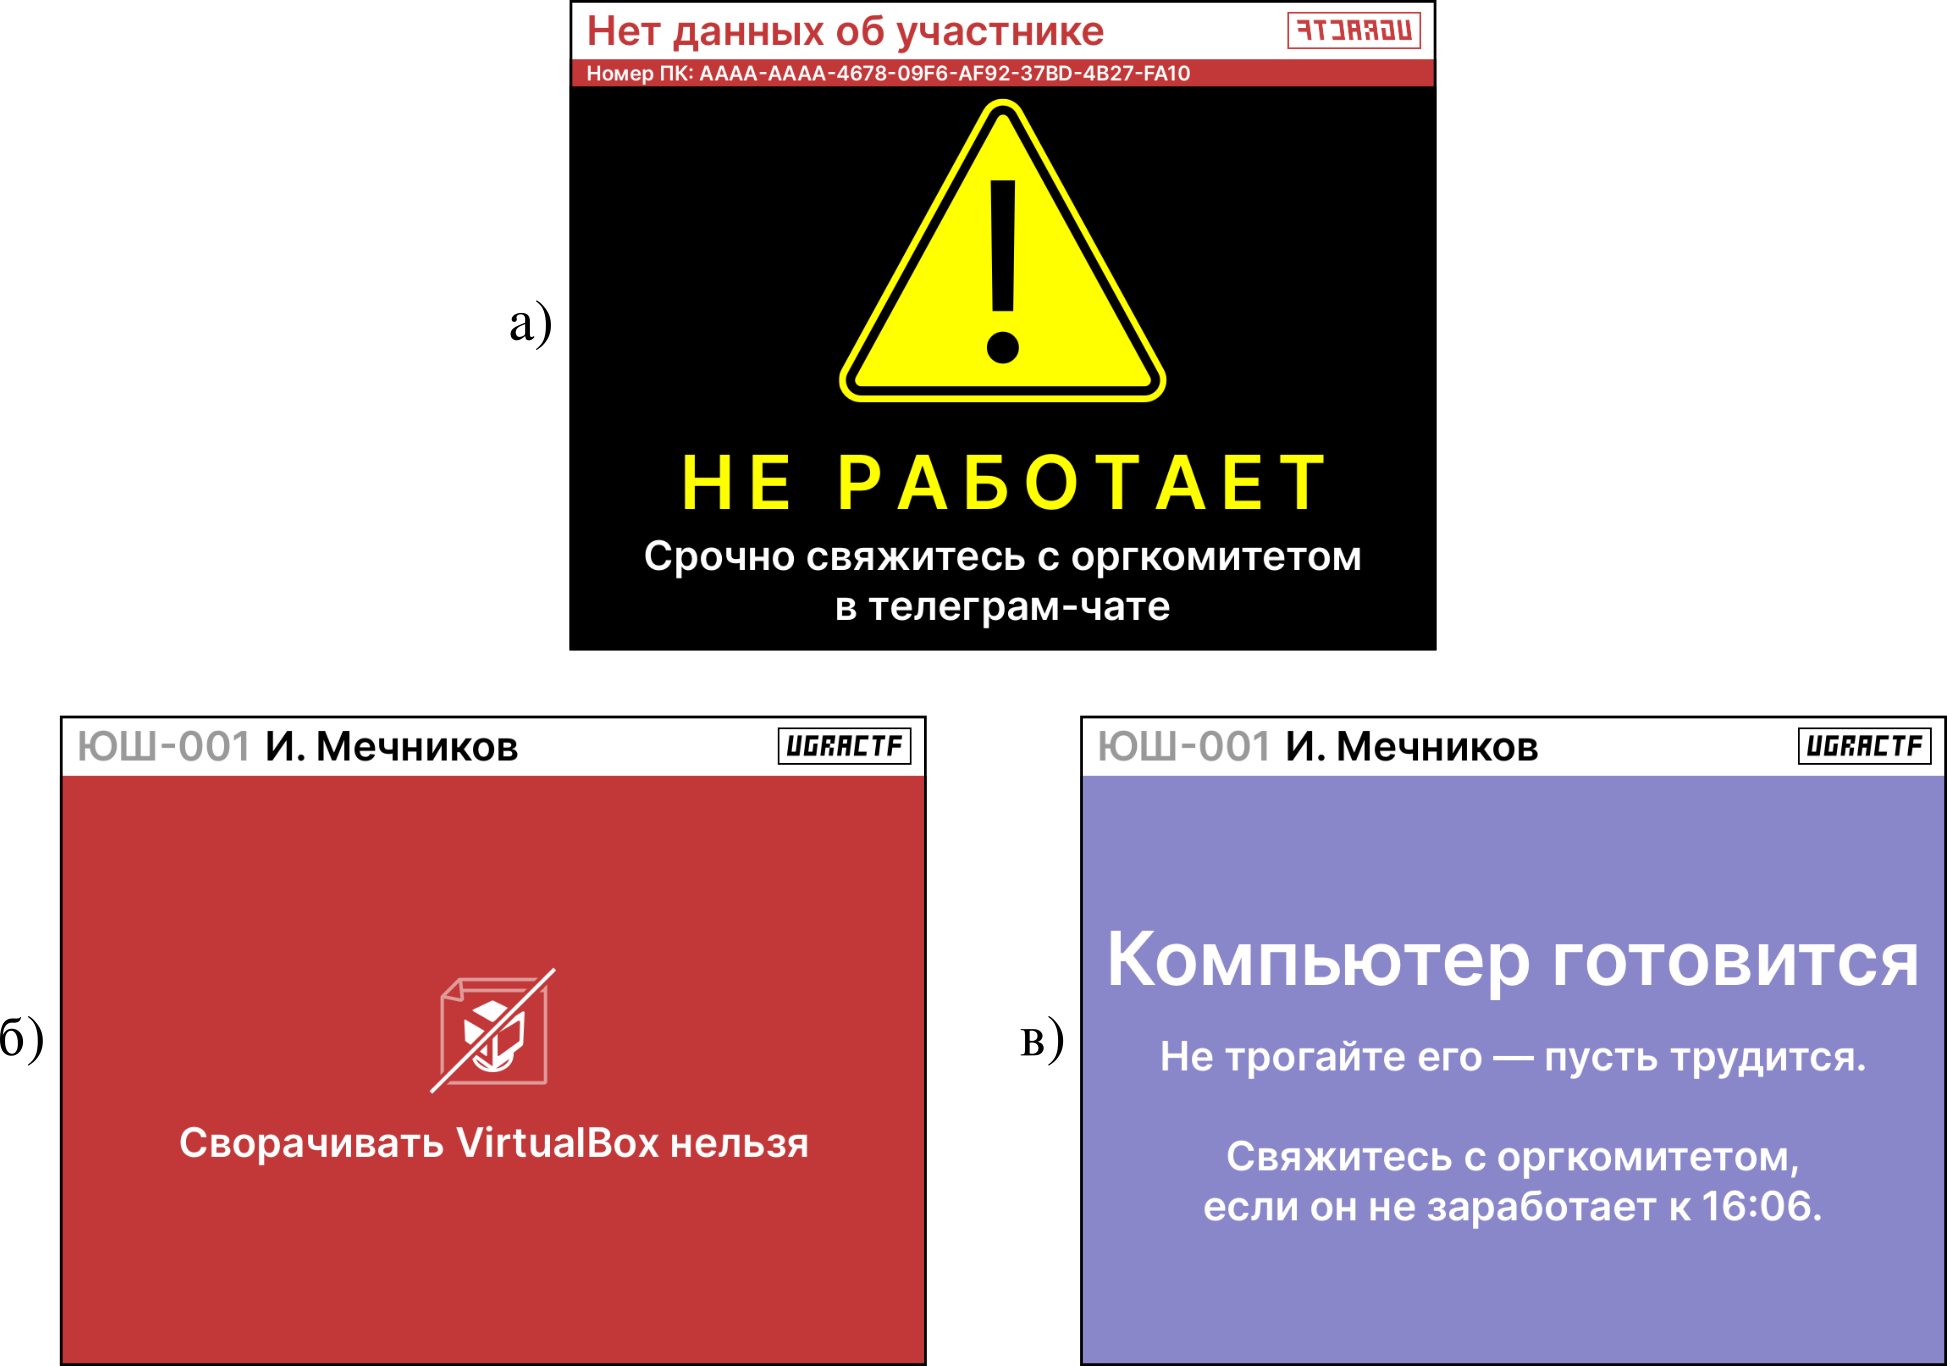
\includegraphics[width=1\textwidth]{inc/img/walls}
  \caption{Три вида индикации состояния системы: а) произошёл сбой; б) штатный режим работы; в) инициализация системы.}
  \label{fig:walls}
\end{figure}

Изображение может содержать произвольный текст~--- например, инструкцию для участника или наблюдателя в случае сбоя, а также диагностическую информацию. Чтобы упростить процесс рассадки участников за рабочие места, изображение также содержит фамилию и инициал участника и его шифр, набранные крупным текстом.

Красный фон изображения выбран неслучайно~--- по правилам олимпиады сворачивать ВМ с гостевой ОС нельзя, и в случае, если это произошло, благодаря яркости цвета, наблюдателю на площадке будет проще заметить данное нарушение.




\section{Модуль среды Kyzylborda}

Для разработки данного модуля применены язык программирования Python и база данных PostgreSQL. Выбор пал на эти технологии по причине того, что каждый разработчик оргкомитета хорошо знаком с ними, к тому же, основная ИС оргкомитета, <<Юрт>>, также написана и использованием этого же технологического стека.

Kyzylborda рассчитана за запуск в ОС NixOS и использует возможности, предоставляемые пакетным менеджером Nix для автоматической изолированной публикации ресурсов при игровых задачах.


\subsection{Модель данных}

Основная сущность в Kyzylborda~--- \texttt{users}. Она содержит в себе сведения для аутентификации участника, его идентификатор и прочие атрибуты.

\begin{figure}[h!]
  \centering
  \includegraphics[width=1\textwidth]{inc/dia/kyzyl.eps}
  \caption{Схема моделей и их отношений в базе данных Kyzylborda}
  \label{fig:kyzyl}
\end{figure}

Все остальные сущности привязаны к \texttt{users} (рисунок \ref{fig:kyzyl}).

Эти сущности связаны с непосредственными функциями, которые должна выполнять борда:
\begin{itemize}
\item \texttt{submitted\_flags} соответствует посылкам участников;
\item \texttt{generated\_tasks}~--- сгенерированным бордой вариантам игровых задач;
\item \texttt{generated\_flags}~--- флагам для этих \texttt{generated\_tasks};
\item \texttt{granted\_hints}~--- подсказкам (не используются в рамках текущего набора правил);
\end{itemize}



\subsection{Пользователь}

Пользователь обладает уникальным идентификатором, благодаря которому можно привязывать к нему другие сущности. Это необходимо для того, чтобы генерировать задачи по вариантам и определять авторов посылок для их оценки, составления рейтинга и~--- после испытания~--- предоставления итоговой отчётности.

Пользователь может быть организатором. Организатор видит в веб-интерфейсе дополнительные поля, содержащие диагностическую информацию, а также может сбрасывать кэш сгенерированных вариантов игровых задач. Посылки организатора проверяются, однако в рейтинге он не учитывается~--- это даёт возможность тестировать задачи прямо во время игры, не мешая участникам.

Пользователь также может быть дисквалифицирован. В этом случае он исключается из рейтинга, а в турнирной таблице возле его строки появляется соответствующая отметка.

Сущность пользователя определяет механизм аутентификации и авторизации, с помощью которого участник может воспользоваться веб-интерфейсом. Это может быть как авторизация по токену, которые загружаются в борду из ИС <<Юрт>>, так и более универсальная авторизация по паре логин-пароль на случай проведения CTF-соревнований, не относящихся к циклу Ugra CTF.

Наконец, пользователю можно присвоить одну или несколько меток~--- текстовых строк, с помощью которых можно как угодно делить участников на группы: например, по площадкам или виду зачёта (в отборочном этапе существует неофициальный зачёт для людей, которые не учатся в школе).

\subsection{Игровые задачи}

Игровые задачи борда принимает в виде директорий особой структуры. Рассмотрим её на конкретном примере~--- динамической задачи.

Эта задача~--- пример того, как можно использовать пакетный менеджер Nix, чтобы создавать нужное программное окружение. В качестве примера задача динамически запускает тривиальное веб-приложение на языке Python, использующее стороннюю зависимость~--- сервер Redis, а также создаёт во вложениях текстовый файл, содержащий косвенный идентификатор участника.

Она также генерирует динамические флаги.

Данные задачи хранятся внутри директории \texttt{tasks}. Структура директории нашей задачи, которая называется \texttt{nix-example}, видна на рисунке \ref{fig:tree}. В первую очередь задача определяется конфигурационным файлом вида \texttt{<название задачи>.yaml}. Он приведён ниже.

\begin{figure}[hb!]
  \centering
  \begin{verbatim}
                      nix-example
                      |-- app
                      |   |-- isolated_run_daemon.sh
                      |   |-- redis.conf
                      |   |-- run_daemon.sh
                      |   \-- server.py
                      |-- generator.py
                      |-- nix-example.yaml
                      \-- run_generator.sh
  \end{verbatim}
  \caption{Демонстрация страницы сгенерированной по варианту пользователя динамической игровой задачи: её страница и вложение}
  \label{fig:tree}
\end{figure}

\begin{lstlisting}[caption={Конфигурационный файл задачи \texttt{nix-example}}]
category:  lol   # категория задачи
points:    100   # стоимость в очках
author:    you   # имя или ник автора
title:     Nix-generated Task   # полное название для интерфейса
description: <p>So it goes.     # описание (HTML)

generator: ./run_generator.sh   # путь к генератору флагов

# описание фонового процесса - сервера веб-приложения
daemon:
    exec: ./run_daemon.sh   # путь к скрипту, запускающему сервер
    cwd: app                # рабочая директория сервера
    socket: app.sock        # серверу нужен выделенный сокет...
    socket_type: http       #   для обмена по протоколу HTTP
\end{lstlisting}

В конфигурационном файле перечислены все сведения, необходимые для того, чтобы сгенерировать флаги, описание и вложения задачи, а также запустить фоновый процесс. Остальные данные в директории задачи~--- непосредственно, программа-генератор и код веб-приложения.

Генератор~--- программа, принимающая на вход косвенный идентификатор пользователя и путь до директории для вложений. Она может создавать и записывать файлы в эту директорию. Генератор всегда возвращает JSON-объект со следующими полями:

\begin{itemize}
\item \texttt{flags}: уникальные флаги для этого варианта задачи;
\item \texttt{substitutions}: данные для подстановки в переменные, которые можно использовать в текстовом описании задачи;
\item \texttt{urls}:  ссылки на сопутствующие ресурсы (в нашем случае~--- на веб-сервер).
\end{itemize}

Код генератора этой задачи тривиален: он создаёт во вложениях файл, записывает в него полученный от борды косвенный идентификатор участника и формирует JSON-объект согласно описанной выше спецификации.

Скрипт, запускающий сервер~--- это исполняемый файл, приведённый ниже.

\begin{lstlisting}[caption={Скрипт, запускающий сервер}]
#!/usr/bin/env nix-shell
#!nix-shell -i bash -p python3 -p python3Packages.flask -p python3Packages.redis -p python3Packages.gunicorn -p redis

statedir="$1"
task_name="$2"

export BWRAP_PROPAGATE_MOUNTS="/bin /usr/bin /nix/store"
exec kyzylborda-isolate \
  --unshare-net \
  --bind "$1" "/state" \
  --bind "$TMPDIR" "/tmp" \
  --ro-bind "$PWD" "$PWD" \
  --chdir "$PWD" \
  -- ./isolated_run_daemon.sh
\end{lstlisting}

Он выполняется не командной оболочкой ОС, а утилитой \texttt{nix-shell}, что следует из первой строки. Вторая строка сообщает утилите, что мы хотим получить чистое программное окружение, содержащее пакеты: \texttt{python3}, \texttt{flask}, \texttt{redis}, \texttt{gunicorn}, которые необходимы для запуска веб-приложения. Наконец, скрипт использует программу Bubblewrap \cite{Bubblewrap}, с помощью которой создаётся изолированный контекст для процесса веб-сервера: он отделён от сетевых интерфейсов ОС и её файловой системы, за исключением рабочей директории, в которой содержатся его ресурсы и директории для временных файлов.

\begin{figure}[h!]
  \centering
  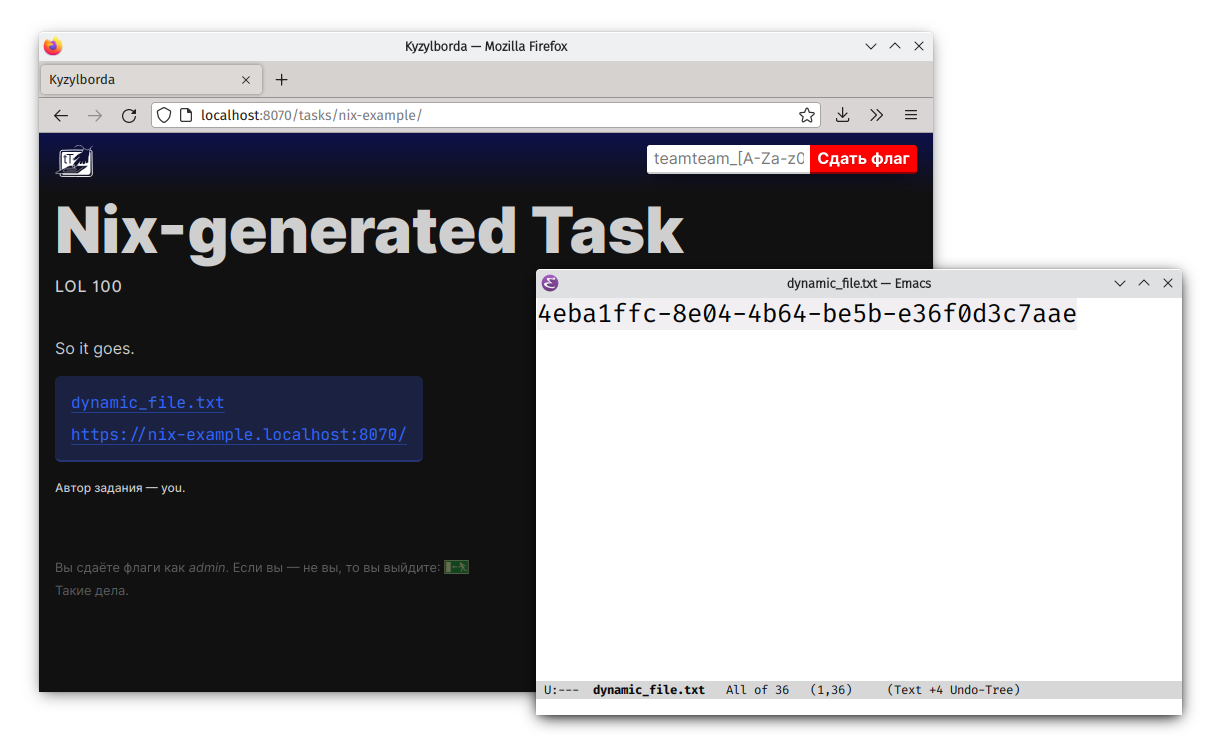
\includegraphics[width=0.92\textwidth]{inc/img/nix}
  \caption{Демонстрация страницы сгенерированной по варианту пользователя динамической игровой задачи: её страница и вложение}
  \label{fig:nix}
\end{figure}

Кроме запуска скрипта борда также автоматически обеспечивает корректную конфигурацию самого сервера~--- начинает принимать HTTP-трафик по адресу: \texttt{nix-example.<домен соревнований>} и перенаправлять его процессу веб-сервера, обеспечивая его доступность во внешней сети.

После размещения задачи в нужной директории и запуска борды, можно воспользоваться веб-интерфейсом, чтобы проверить, что задача, во-первых, начала отображаться в интерфейсе, во-вторых, при переходе на её страницу действительно генерируется вариант для текущего пользователя, соответствующий формальному описанию задачи (рисунок \ref{fig:nix}).

За запуск и остановку процессов отвечает системная служба \texttt{supervisord} \cite{supervisord}. В ней реализованы безопасные и надёжные механизмы управления задачами, и она предоставляет возможность управления посредством программного интерфейса. Благодаря использованию этой технологии и введению корректных абстракций в коде модуля Kyzylboard, процессы, связанные с задачами, могут использовать в целях изоляции и обеспечения воспроизводимой программной среды не только Nix, но и технологии контейнеризации, например, Docker \cite{Docker}.


\subsection{Интерфейс}

Для веб-интерфейса используется библиотеку Flask \cite{Flask}. Она позволяет создать веб-сервер и определить его поведение: создать т.н. маршруты \textit(англ. routes)~--- правила, которые определяют, как обрабатывать тот или иной HTTP-запрос в зависимости от его типа или содержимого.

Интерфейс рассчитан на использование в браузере. Код страниц для браузера формируется из шаблонов, логика которых изолирована от основной логики модуля Kyzylborda. Это согласуется с принципами модульной архитектуры, описанными в Главе 2.

С помощью веб-интерфейса участники получают доступ к турнирной таблице, описаниям задач и сдают свои посылки. Все посылки принимаются веб-сервером и записываются в базу данных как сущности типа \texttt{submitted\_flags}.



\section{Выводы}

В данной главе была рассмотрена подробная модель автоматизированной системы, предоставляющей среду для проведения дистанционных испытаний в области защиты информации, отражающая структуру её программных компонент.

В результате проведённой работе были разработаны два основных модуля системы и изучены особенности, связанные с их реализацией.
